\documentclass[conference]{IEEEtran}

\usepackage{amsmath,amssymb,amsfonts}
\usepackage{amsthm}
\usepackage{algorithmic}
\usepackage{algorithm}

% Theorem environments
\newtheorem{theorem}{Theorem}
\newtheorem{lemma}[theorem]{Lemma}
\newtheorem{corollary}[theorem]{Corollary}
\newtheorem{definition}{Definition}
\newtheorem{axiom}{Axiom}
\usepackage{graphicx}
\usepackage{textcomp}
\usepackage{xcolor}
\usepackage{booktabs}
\usepackage{multirow}
\usepackage{tikz}
\usepackage{hyperref}
\usepackage{cleveref}

\usetikzlibrary{shapes,arrows,positioning,fit,calc,decorations.pathreplacing}

% Custom commands
\newcommand{\mapfhet}{\textsc{MAPF-HET}}
\newcommand{\ekkor}{\textsc{EK-KOR2}}
\newcommand{\mixedcbs}{\textsc{Mixed-CBS}}
\newcommand{\ecbs}{\textsc{E-CBS}}
\newcommand{\hybridcbs}{\textsc{Hybrid-CBS}}
\newcommand{\deadline}{\textsc{Deadline-CBS}}

\begin{document}

\title{From Planning to Execution: Heterogeneous Multi-Agent Path Finding with Field-Centric Distributed Coordination}

\author{
\IEEEauthorblockN{Bojan Janjatovi\'{c}}
\IEEEauthorblockA{\textit{Elektrokombinacija} \\
Kikinda, Serbia \\
bojan.janjatovic@gmail.com}
}

\maketitle

\begin{abstract}
Coordinating heterogeneous robot fleets operating in different dimensional spaces—1D rails, 2D floors, 3D airspace—presents challenges that existing Multi-Agent Path Finding (MAPF) formulations do not address. We introduce Mixed-Dimensional MAPF (MD-MAPF), the first MAPF formulation with a dimensionality function mapping agents to operational spaces and a vertex compatibility function constraining spatial access. We present a six-class dimensional conflict taxonomy (LINEAR, PLANAR, CROSSING, AERIAL, VERTICAL, AIR-GROUND) with specialized resolution strategies achieving 5.6$\times$ speedup over baseline CBS. To bridge planning and execution, we map deadline slack to field components in the EK-KOR2 distributed coordination layer, enabling gradient-based resource allocation that respects planning constraints. Drawing from collective behavior research, we implement $k=7$ topological neighbor coordination that maintains scale-free correlations across 500-2000 module installations, achieving $O(\log N)$ convergence with 42\% CAN-FD bandwidth utilization. Experimental evaluation demonstrates 99.9\% deadline compliance and zero energy violations over 24-hour operational cycles. The implementation comprises 7K lines of Go for planning with dual C/Rust embedded targets for execution.
\end{abstract}


\section{Introduction}
\label{sec:intro}

Coordinating heterogeneous robot fleets presents fundamental challenges that existing Multi-Agent Path Finding (MAPF) formulations do not address. Consider a robotic battery swap station for electric buses: mobile robots navigate the 2D floor, rail-mounted manipulators operate along 1D tracks, and inspection drones traverse 3D airspace. These agents interact at shared handoff points, compete for charging resources, and must meet strict operational deadlines. Standard MAPF algorithms~\cite{sharon2015cbs,stern2019mapf} assume homogeneous agents operating in the same space, leaving this heterogeneous coordination problem unsolved.

This paper bridges two research areas: MAPF planning with optimality guarantees and distributed real-time execution with scalability requirements. We present \mapfhet{}, a unified framework spanning from abstract planning to embedded coordination.

\subsection{Motivating Application}

Electric bus depot charging exemplifies the heterogeneous coordination challenge. A typical installation includes:
\begin{itemize}
    \item \textbf{500-2000 power modules} (3.3 kW each) forming reconfigurable charging points
    \item \textbf{Rail robots} for heavy battery transport along fixed tracks
    \item \textbf{Mobile robots} for auxiliary logistics on the depot floor
    \item \textbf{Drones} for inspection and light-payload delivery
\end{itemize}

These agents operate in fundamentally different dimensional spaces yet must coordinate at shared resources. A rail robot cannot deviate from its track to avoid a mobile robot; a drone must land at designated pads to interact with ground systems. Existing MAPF formulations cannot capture these dimensional constraints.

Furthermore, the power modules themselves require coordination: load balancing across the grid connection, thermal management, and deadline-driven charging sessions. This creates a second layer of multi-agent coordination below the robotic planning layer.

\subsection{Contributions}

This paper makes four contributions:

\textbf{1. MD-MAPF Formulation:} We introduce Mixed-Dimensional MAPF, the first MAPF formulation with a dimensionality function $\kappa(a) \rightarrow \{1, 2, 3\}$ mapping agents to 1D rail, 2D mobile, or 3D aerial operational spaces. The vertex compatibility function $\delta(v)$ constrains which agents can access which locations, enabling precise modeling of dimensional restrictions.

\textbf{2. Six-Class Dimensional Conflict Taxonomy:} We classify conflicts by dimensional interaction: LINEAR (1D-1D), PLANAR (2D-2D), CROSSING (1D-2D), AERIAL (3D-3D same layer), VERTICAL (3D-3D across layers), and AIR-GROUND (3D-1D/2D). Each class admits specialized resolution strategies that exploit dimensional structure, significantly pruning the CBS search tree.

\textbf{3. Planning-Execution Unification:} We bridge the gap between optimal MAPF planning and real-time distributed execution. Deadline slack from the planning layer maps to field components in the execution layer, enabling gradient-based coordination that respects planning constraints while adapting to runtime conditions.

\textbf{4. Bio-Inspired Scale-Free Coordination:} Drawing from collective behavior research~\cite{cavagna2010scale}, we implement $k=7$ topological neighbor coordination that maintains scale-free correlations across 500-2000 module installations. Information propagates in $O(\log N)$ hops regardless of physical network topology.

\subsection{Paper Organization}

Section~\ref{sec:related} surveys related work in MAPF, energy-aware planning, and distributed systems. Section~\ref{sec:problem} formalizes MD-MAPF, the conflict taxonomy, and the execution model. Section~\ref{sec:algorithms} presents our CBS variants: \mixedcbs{}, \ecbs{}, \deadline{}, and \hybridcbs{}. Section~\ref{sec:ekkor2} describes the \ekkor{} execution layer with potential field scheduling and topological coordination. Section~\ref{sec:theory} establishes theoretical properties. Section~\ref{sec:implementation} details implementation in Go (7K LOC) with C/Rust embedded targets. Section~\ref{sec:evaluation} presents experimental results. Section~\ref{sec:conclusion} concludes.


\section{Related Work}
\label{sec:related}

We survey four areas: MAPF formulations for heterogeneous agents, conflict classification in CBS, energy-aware planning, and distributed coordination systems.

\subsection{Multi-Agent Path Finding}

The foundational CBS algorithm~\cite{sharon2015cbs} introduced two-level search: high-level conflict detection and low-level single-agent planning. Subsequent work improved efficiency through enhanced heuristics (CBSH~\cite{felner2018cbsh}), improved conflict classification (ICBS~\cite{boyarski2015icbs}), and continuous-time extensions (CCBS~\cite{andreychuk2022ccbs}).

\textbf{Heterogeneous MAPF:} G-MAPF~\cite{atzmon2020gmapf} generalizes agent representation with state-based transition functions but assumes all agents operate on the same graph structure. LA-MAPF~\cite{li2019lamapf} handles geometric agents with varying footprints but not dimensional restrictions. Multi-Train Path Finding~\cite{atzmon2019trains} addresses 1D rail networks in isolation. The Flatland Challenge~\cite{li2021flatland} demonstrated scalable rail planning but without integration with 2D/3D agents.

\textbf{Gap:} No existing work models agents operating in fundamentally different dimensional spaces (1D rail, 2D ground, 3D aerial) within a unified MAPF formulation. MD-MAPF introduces the dimensionality function $\kappa(a) \rightarrow \{1,2,3\}$ and vertex compatibility function $\delta(v)$ to address this gap.

\subsection{Conflict Classification}

Conflict classification in MAPF literature follows three approaches:
\begin{itemize}
    \item \textbf{Basic:} CBS~\cite{sharon2015cbs} defines only vertex and edge conflicts without structural distinction
    \item \textbf{Cost-Based:} ICBS~\cite{boyarski2015icbs} introduced cardinal/semi-cardinal/non-cardinal classification based on cost impact using MDDs
    \item \textbf{Pattern-Based:} Pairwise symmetry reasoning~\cite{li2021symmetry} recognizes corridor, rectangle, and target symmetry patterns, achieving up to 4 orders of magnitude runtime improvement
\end{itemize}

Our six-class taxonomy (LINEAR, PLANAR, CROSSING, AERIAL, VERTICAL, AIR-GROUND) uses a fundamentally different classification principle based on dimensional interaction. The CROSSING, VERTICAL, and AIR-GROUND classes have no prior treatment in the literature.

\subsection{Energy-Aware Planning}

Energy constraints are well-studied in vehicle routing. NRHF-MAPF~\cite{scott2024nrhf} extends CBS for hybrid-fuel UAVs with battery and noise restrictions but does not include automatic charging waypoint insertion. MO-CBS~\cite{ren2021mocbs} treats energy as an optimization objective rather than a hard constraint. The Electric Vehicle Routing Problem literature (EVRPTW~\cite{schneider2014evrptw}) provides mature charging integration but operates in VRP frameworks without collision avoidance.

\textbf{Gap:} E-CBS differs from prior work by treating battery constraints as hard limits, performing automatic charging station waypoint insertion during conflict resolution, and using action-specific energy models (hover/move/climb/descend) unified within CBS.

\subsection{Airspace Management}

Labib et al.~\cite{labib2019airspace} present a multilayer low-altitude airspace model dividing Class G airspace into horizontal layers with inter-layer transitions. The METROPOLIS project~\cite{sunil2015metropolis} tested layers segmented by travel direction. UTM/U-space frameworks~\cite{nasa2020utm,faa2023uam} provide operational concepts but leave internal layering to implementation.

Our model adds: (1) functional layer naming with operational semantics (ground/handoff/work/transit), (2) exclusive vertical corridors as the only transition points, and (3) MAPF integration for collision-free path planning within the layered structure.

\subsection{Distributed Coordination}

Collective behavior research provides theoretical foundation for our coordination approach. Cavagna et al.~\cite{cavagna2010scale} demonstrated that starling flocks maintain scale-free correlations through topological (not metric) neighbor interaction with $k \approx 6$-7 neighbors.

Potential field methods originated in robotics~\cite{khatib1986potential} for obstacle avoidance. We adapt these to temporal scheduling, where task deadlines create attractive potentials and resource contention creates repulsive fields.

Distributed consensus protocols (Paxos~\cite{lamport1998paxos}, Raft~\cite{ongaro2014raft}) provide foundations for our threshold consensus, adapted for embedded systems with Byzantine fault tolerance and density-dependent activation.

Real-time scheduling theory~\cite{sha1990priority,buttazzo2011real} informs our deadline handling, though we replace priority inheritance with field-mediated coordination for improved scalability.

\subsection{Commercial Systems}

Amazon Robotics coordinates heterogeneous fleets (Proteus, Titan, Hercules, Sequoia, Cardinal) through their DeepFleet system managing over 1 million robots. Geek+ and Locus Robotics support mixed navigation types through unified management platforms.

These systems differ from our approach: they use heuristic methods without formal optimality guarantees, handle heterogeneity through separate planning modules rather than unified formulations, and don't address the 1D/2D/3D dimensional distinctions central to MD-MAPF.

Ocado Technology demonstrates automated battery swap (sub-one-minute hot swaps, 12-minute charge cycles, 7\%+ increased utilization) within their proprietary grid system, validating commercial viability of energy-aware automation.


\section{Problem Formulation}
\label{sec:problem}

This section presents the Mixed-Dimensional MAPF (MD-MAPF) formulation, the dimensional conflict taxonomy, and the execution model that bridges planning to real-time coordination.

\subsection{Mixed-Dimensional MAPF (MD-MAPF)}

\begin{definition}[MD-MAPF Instance]
A mixed-dimensional MAPF problem is defined as a tuple:
\begin{equation}
\mathcal{I} = (G, A, T, \kappa, \delta)
\end{equation}
where:
\begin{itemize}
    \item $G = (V, E)$ is a workspace graph with vertices $V$ and edges $E$
    \item $A = \{a_1, a_2, \ldots, a_n\}$ is a set of agents
    \item $T = \{t_1, t_2, \ldots, t_m\}$ is a set of tasks with deadlines
    \item $\kappa: A \rightarrow \{1, 2, 3\}$ is an agent dimensionality function
    \item $\delta: V \rightarrow \mathcal{P}(\{1, 2, 3\})$ is a vertex accessibility function
\end{itemize}
\end{definition}

The dimensionality function $\kappa(a)$ determines the operational space of each agent:

\begin{table}[htbp]
\centering
\caption{Agent Dimensionality Classification}
\label{tab:dimensionality}
\begin{tabular}{@{}cll@{}}
\toprule
$\kappa(a)$ & Type & Motion Space \\
\midrule
1 & Rail Robot & 1D linear path \\
2 & Mobile Robot & 2D planar surface \\
3 & Drone & 3D volumetric space \\
\bottomrule
\end{tabular}
\end{table}

\begin{definition}[Vertex Compatibility]
Agent $a$ can occupy vertex $v$ if and only if $\kappa(a) \in \delta(v)$.
\end{definition}

This formalizes that rail robots access only rail vertices, mobile robots access floor vertices, and drones access airspace vertices at appropriate altitude layers.

\begin{figure}[htbp]
\centering
% MD-MAPF Workspace: 1D rails, 2D floor, 3D airspace
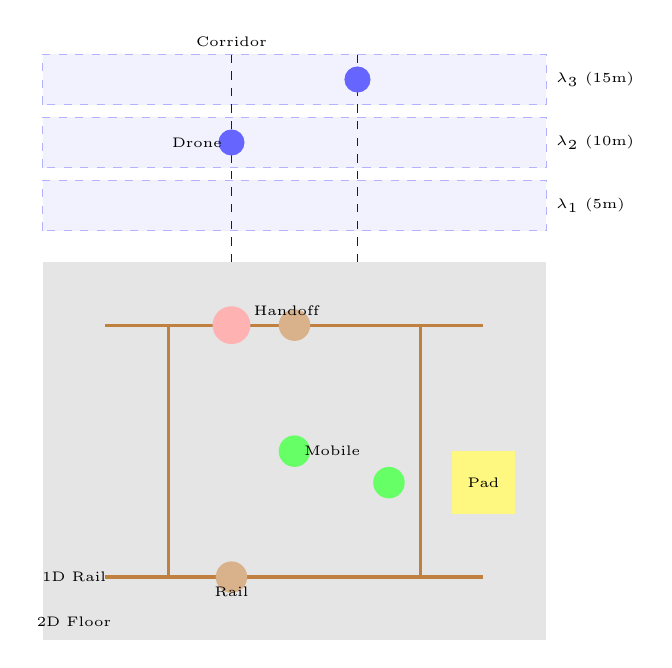
\begin{tikzpicture}[
    scale=0.8,
    rail/.style={very thick, brown},
    floor/.style={fill=gray!20},
    airspace/.style={fill=blue!5, draw=blue!30, dashed},
    agent1d/.style={fill=brown!60, circle, minimum size=0.4cm},
    agent2d/.style={fill=green!60, circle, minimum size=0.4cm},
    agent3d/.style={fill=blue!60, circle, minimum size=0.3cm}
]

% Floor (2D layer)
\fill[floor] (0,0) rectangle (8,6);
\node at (0.5, 0.3) {\tiny 2D Floor};

% Rails (1D)
\draw[rail] (1, 1) -- (7, 1);
\draw[rail] (1, 5) -- (7, 5);
\draw[rail] (2, 1) -- (2, 5);
\draw[rail] (6, 1) -- (6, 5);
\node at (0.5, 1) {\tiny 1D Rail};

% Airspace layers
\begin{scope}[yshift=6.5cm]
    \fill[airspace] (0, 0) rectangle (8, 0.8);
    \node[right] at (8, 0.4) {\tiny $\lambda_1$ (5m)};
    \fill[airspace] (0, 1) rectangle (8, 1.8);
    \node[right] at (8, 1.4) {\tiny $\lambda_2$ (10m)};
    \fill[airspace] (0, 2) rectangle (8, 2.8);
    \node[right] at (8, 2.4) {\tiny $\lambda_3$ (15m)};
\end{scope}

% Vertical corridors
\draw[dashed, blue] (3, 6) -- (3, 9.3);
\draw[dashed, blue] (5, 6) -- (5, 9.3);
\node at (3, 9.5) {\tiny Corridor};

% Agents
\node[agent1d] (r1) at (3, 1) {};
\node[agent1d] (r2) at (4, 5) {};
\node[agent2d] (m1) at (4, 3) {};
\node[agent2d] (m2) at (5.5, 2.5) {};
\node[agent3d] (d1) at (3, 7.9) {};
\node[agent3d] (d2) at (5, 8.9) {};

% Labels
\node[below] at (r1) {\tiny Rail};
\node[right] at (m1) {\tiny Mobile};
\node[left] at (d1) {\tiny Drone};

% Handoff point
\fill[red!30] (3, 5) circle (0.3);
\node[above right] at (3.2, 5) {\tiny Handoff};

% Charging pad
\fill[yellow!50] (6.5, 2) rectangle (7.5, 3);
\node at (7, 2.5) {\tiny Pad};

\end{tikzpicture}

\caption{MD-MAPF workspace showing 1D rails (brown), 2D floor (gray), 3D airspace layers ($\lambda_1$-$\lambda_3$), vertical corridors, handoff points, and charging pads.}
\label{fig:workspace}
\end{figure}

\subsection{Space-Time Representation}

\begin{definition}[Space-Time State]
For an agent of dimensionality $d$, the state in the space-time graph is:
\begin{equation}
s = (v, t, \lambda) \quad \text{where} \quad v \in V, t \in \mathbb{R}_{\geq 0}, \lambda \in \Lambda
\end{equation}
\end{definition}

The layer component $\lambda$ has dimension-specific semantics:
\begin{itemize}
    \item For $d = 1$: $\lambda$ is position on rail segment (continuous)
    \item For $d = 2$: $\lambda = \emptyset$ (not applicable)
    \item For $d = 3$: $\lambda \in \{0, 5, 10, 15\}$ meters (discrete altitude layers)
\end{itemize}

\begin{axiom}[Dimensionality Conservation]
An agent cannot change its dimensionality during execution:
\begin{equation}
\forall a \in A, \forall t_1, t_2 \in \mathbb{R}_{\geq 0}: \kappa(a, t_1) = \kappa(a, t_2)
\end{equation}
\end{axiom}

\begin{axiom}[Inter-Dimensional Transition]
An agent of dimension $d_1$ can interact with an agent of dimension $d_2$ only at vertices where their dimensions intersect:
\begin{equation}
\text{interact}(a_1, a_2, v) \Rightarrow \kappa(a_1) \in \delta(v) \land \kappa(a_2) \in \delta(v)
\end{equation}
\end{axiom}

\subsection{Dimensional Conflict Taxonomy}

Classical CBS~\cite{sharon2015cbs} treats all conflicts uniformly. We introduce a six-class taxonomy based on dimensional interaction, enabling specialized resolution strategies.

\begin{definition}[Dimensional Conflict]
Let $a_1, a_2 \in A$ be agents with dimensionalities $d_1 = \kappa(a_1)$ and $d_2 = \kappa(a_2)$. A conflict between them is classified by the pair $(d_1, d_2)$.
\end{definition}

\begin{table}[htbp]
\centering
\caption{Six-Class Dimensional Conflict Taxonomy}
\label{tab:conflicts}
\begin{tabular}{@{}clll@{}}
\toprule
Class & $(d_1, d_2)$ & Name & Description \\
\midrule
$C_1$ & $(1, 1)$ & \textsc{Linear} & Same rail segment \\
$C_2$ & $(2, 2)$ & \textsc{Planar} & 2D plane collision \\
$C_3$ & $(1, 2)$ & \textsc{Crossing} & Rail-floor intersection \\
$C_4$ & $(3, 3)$ & \textsc{Aerial} & Same airspace layer \\
$C_5$ & $(3, 3)$ & \textsc{Vertical} & Vertical corridor \\
$C_6$ & $(3, 1/2)$ & \textsc{Air-Ground} & Handoff point \\
\bottomrule
\end{tabular}
\end{table}

Each conflict class admits specialized resolution strategies that exploit dimensional structure, achieving significant pruning of the CBS search tree compared to uniform treatment.

\begin{figure}[htbp]
\centering
% Conflict Taxonomy: 6 conflict classes visual grid
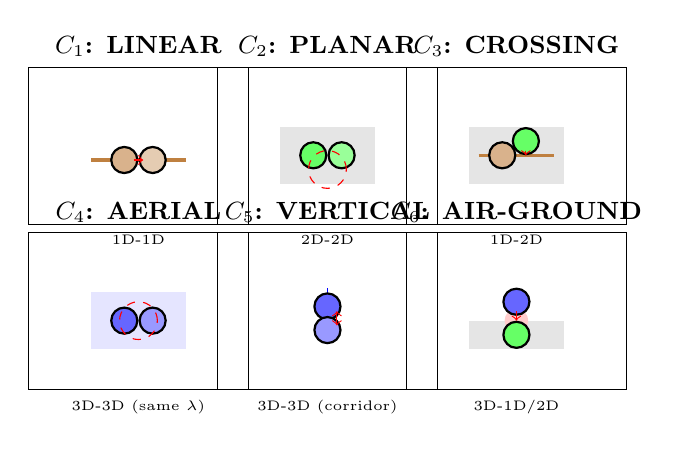
\begin{tikzpicture}[
    scale=0.6,
    box/.style={draw, minimum width=2.8cm, minimum height=2cm, align=center},
    agent/.style={circle, minimum size=0.3cm, draw, thick}
]

% Row 1
\node[box] (c1) at (0, 0) {};
\node[above] at (c1.north) {\small\textbf{$C_1$: LINEAR}};
\draw[brown, very thick] (-1, -0.3) -- (1, -0.3);
\node[agent, fill=brown!60] at (-0.3, -0.3) {};
\node[agent, fill=brown!40] at (0.3, -0.3) {};
\draw[red, ->] (-0.1, -0.3) -- (0.1, -0.3);
\node[below] at (c1.south) {\tiny 1D-1D};

\node[box] (c2) at (4, 0) {};
\node[above] at (c2.north) {\small\textbf{$C_2$: PLANAR}};
\fill[gray!20] (3, -0.8) rectangle (5, 0.4);
\node[agent, fill=green!60] at (3.7, -0.2) {};
\node[agent, fill=green!40] at (4.3, -0.2) {};
\draw[red, dashed] (4, -0.5) circle (0.4);
\node[below] at (c2.south) {\tiny 2D-2D};

\node[box] (c3) at (8, 0) {};
\node[above] at (c3.north) {\small\textbf{$C_3$: CROSSING}};
\fill[gray!20] (7, -0.8) rectangle (9, 0.4);
\draw[brown, very thick] (7.2, -0.2) -- (8.8, -0.2);
\node[agent, fill=brown!60] at (7.7, -0.2) {};
\node[agent, fill=green!60] at (8.2, 0.1) {};
\draw[red, ->] (8.2, -0.1) -- (8.2, -0.2);
\node[below] at (c3.south) {\tiny 1D-2D};

% Row 2
\node[box] (c4) at (0, -3.5) {};
\node[above] at (c4.north) {\small\textbf{$C_4$: AERIAL}};
\fill[blue!10] (-1, -4.3) rectangle (1, -3.1);
\node[agent, fill=blue!60] at (-0.3, -3.7) {};
\node[agent, fill=blue!40] at (0.3, -3.7) {};
\draw[red, dashed] (0, -3.7) circle (0.4);
\node[below] at (c4.south) {\tiny 3D-3D (same $\lambda$)};

\node[box] (c5) at (4, -3.5) {};
\node[above] at (c5.north) {\small\textbf{$C_5$: VERTICAL}};
\draw[blue, dashed] (4, -4.2) -- (4, -3);
\node[agent, fill=blue!60] at (4, -3.4) {};
\node[agent, fill=blue!40] at (4, -3.9) {};
\draw[red, <->] (4.2, -3.5) -- (4.2, -3.8);
\node[below] at (c5.south) {\tiny 3D-3D (corridor)};

\node[box] (c6) at (8, -3.5) {};
\node[above] at (c6.north) {\small\textbf{$C_6$: AIR-GROUND}};
\fill[gray!20] (7, -4.3) rectangle (9, -3.7);
\fill[red!20] (8, -3.7) circle (0.25);
\node[agent, fill=blue!60] at (8, -3.3) {};
\node[agent, fill=green!60] at (8, -4) {};
\draw[red, ->] (8, -3.5) -- (8, -3.7);
\node[below] at (c6.south) {\tiny 3D-1D/2D};

\end{tikzpicture}

\caption{Six-class dimensional conflict taxonomy. Each class has distinct resolution strategies based on the dimensional interaction between agents.}
\label{fig:conflicts}
\end{figure}

\subsection{Layered Airspace Model}

\begin{definition}[Airspace Layer]
The airspace is divided into discrete functional layers:
\begin{equation}
\Lambda = \{\lambda_0, \lambda_1, \lambda_2, \lambda_3\} = \{0\text{m}, 5\text{m}, 10\text{m}, 15\text{m}\}
\end{equation}
with operational semantics:
\begin{itemize}
    \item $\lambda_0$ (Ground): Landing, charging, handoff operations
    \item $\lambda_1$ (Handoff): Interaction with ground robots
    \item $\lambda_2$ (Work): Primary task execution layer
    \item $\lambda_3$ (Transit): Fast transit without conflicts
\end{itemize}
\end{definition}

\begin{definition}[Vertical Corridor]
A vertical corridor is a set of vertices $C \subset V$ such that:
\begin{equation}
\forall v \in C: \text{is\_corridor}(v) = \text{true}, \quad \forall \lambda \in \Lambda: \exists! v \in C: \text{layer}(v) = \lambda
\end{equation}
\end{definition}

Corridors are the exclusive transition points for layer changes.

\begin{definition}[Layer Transition Matrix]
The permitted layer transitions form matrix $\mathbf{T}$:
\begin{equation}
\mathbf{T} = \begin{bmatrix}
\checkmark & \checkmark & \times & \times \\
\checkmark & \checkmark & \checkmark & \times \\
\times & \checkmark & \checkmark & \checkmark \\
\times & \times & \checkmark & \checkmark
\end{bmatrix}
\end{equation}
where $T_{ij} = \checkmark$ indicates direct transition from $\lambda_i$ to $\lambda_j$ is permitted.
\end{definition}

\begin{axiom}[Corridor Exclusivity]
At any time, at most one drone can occupy a vertical corridor:
\begin{equation}
\forall C \in \text{Corridors}, \forall t: |\{a \in A : \text{position}(a, t) \in C\}| \leq 1
\end{equation}
\end{axiom}

\subsection{Energy Model}

\begin{definition}[Drone Energy State]
The drone state is extended with an energy component:
\begin{equation}
s = (v, t, \lambda, e) \quad \text{where} \quad e \in [0, E_{\max}]
\end{equation}
with $e$ representing remaining energy in Wh and $E_{\max}$ the battery capacity.
\end{definition}

\begin{definition}[Energy Consumption]
For action $\alpha$ with duration $\Delta t$:
\begin{equation}
\text{consume}(\alpha, \Delta t) = P(\alpha) \cdot \Delta t / 3600 \quad [\text{Wh}]
\end{equation}
where $P(\alpha)$ is action-specific power consumption:
\end{definition}

\begin{table}[htbp]
\centering
\caption{Drone Power Consumption Model}
\label{tab:power}
\begin{tabular}{@{}lc@{}}
\toprule
Action $\alpha$ & $P(\alpha)$ [W] \\
\midrule
\textsc{Hover} & 50 \\
\textsc{Move\_Horizontal} & 75 \\
\textsc{Climb} & 125 \\
\textsc{Descend} & 40 \\
\bottomrule
\end{tabular}
\end{table}

\begin{definition}[Path Energy Validity]
Path $\pi = [(v_0, t_0), \ldots, (v_k, t_k)]$ is energy-valid iff:
\begin{equation}
\forall i \in [1, k]: e_i = e_{i-1} - \text{consume}(\alpha_i, t_i - t_{i-1}) > 0
\end{equation}
with recharging at stations: if $\text{is\_charging\_pad}(v_i)$ then $e_i = E_{\max}$.
\end{definition}

\subsection{Deadline-Aware Execution Model}

To bridge planning to execution, we introduce deadline slack as a coordination signal.

\begin{definition}[Deadline Slack]
For task $t$ with deadline $d_t$, estimated duration $\tau_t$, at current time $t_{\text{now}}$:
\begin{equation}
\text{slack}(t) = d_t - (t_{\text{now}} + \tau_t)
\end{equation}
\end{definition}

\begin{definition}[Critical Task]
A task is critical when $\text{slack}(t) < \theta_{\text{critical}}$ (default 10 seconds).
\end{definition}

The slack value is normalized and published as a field component in the \ekkor{} execution layer, enabling gradient-based coordination where modules with tight deadlines naturally attract resources from neighbors with slack capacity.


\section{Algorithm Design}
\label{sec:algorithms}

We present four CBS variants that address different aspects of the MD-MAPF problem: \mixedcbs{} for dimensional conflicts, \ecbs{} for energy constraints, \deadline{} for deadline awareness, and \hybridcbs{} for integrated planning-execution.

\subsection{\mixedcbs{}: Dimensional Conflict Resolution}

\mixedcbs{} extends CBS with dimension-aware conflict classification and specialized resolution strategies.

\begin{algorithm}
\caption{\mixedcbs{} Algorithm}
\label{alg:mixedcbs}
\begin{algorithmic}[1]
\REQUIRE MD-MAPF instance $\mathcal{I}$
\ENSURE Solution $\pi$ or \textsc{Failure}
\STATE $\text{root} \leftarrow \text{compute\_initial\_assignment}(\mathcal{I})$
\STATE $\text{root.paths} \leftarrow \text{plan\_all\_paths}(\text{root}, \mathcal{I})$
\STATE $\text{OPEN} \leftarrow \{\text{root}\}$
\WHILE{$\text{OPEN} \neq \emptyset$}
    \STATE $N \leftarrow \text{extract\_min}(\text{OPEN})$
    \STATE $\text{conflict} \leftarrow \text{find\_first\_conflict}(N.\text{paths})$
    \IF{$\text{conflict} = \emptyset$}
        \RETURN $N$ \COMMENT{Solution found}
    \ENDIF
    \STATE $\text{dim} \leftarrow \text{classify\_dimension}(\text{conflict})$
    \STATE $\text{children} \leftarrow \text{resolve\_by\_dimension}(N, \text{conflict}, \text{dim})$
    \FOR{each child in children}
        \STATE $\text{child.paths} \leftarrow \text{replan\_affected}(\text{child}, \text{conflict.agents})$
        \IF{$\text{child.paths} \neq \emptyset$}
            \STATE $\text{OPEN} \leftarrow \text{OPEN} \cup \{\text{child}\}$
        \ENDIF
    \ENDFOR
\ENDWHILE
\RETURN \textsc{Failure}
\end{algorithmic}
\end{algorithm}

The key innovation is the \texttt{resolve\_by\_dimension} function, which applies conflict-class-specific strategies:

\textbf{Strategy $C_1$ (\textsc{Linear}):} For rail robot conflicts on segment $S$:
\begin{equation}
\text{resolve\_linear}(a_1, a_2, S, t) = \text{constrain}(a_{\text{trailing}}, \text{wait\_at\_junction}, t)
\end{equation}
Rail robots cannot pass on a segment; one must yield at a junction.

\textbf{Strategy $C_2$ (\textsc{Planar}):} Standard CBS branching:
\begin{equation}
\text{resolve\_planar}(a_1, a_2, v, t) = \{\text{constrain}(a_1, v, t), \text{constrain}(a_2, v, t)\}
\end{equation}

\textbf{Strategy $C_3$ (\textsc{Crossing}):} Rail-mobile intersection with priority to rail (higher inertia):
\begin{equation}
\text{resolve\_crossing}(a_{\text{rail}}, a_{\text{mobile}}, v, t) = \{\text{constrain}(a_{\text{mobile}}, v, [t-\epsilon, t+\epsilon])\}
\end{equation}

\textbf{Strategy $C_4$ (\textsc{Aerial}):} Similar to planar but in 3D layer context.

\textbf{Strategy $C_5$ (\textsc{Vertical}):} Corridor exclusivity forces sequentialization:
\begin{equation}
\text{resolve\_vertical}(a_1, a_2, C, t) = \text{constrain}(a_{\text{following}}, C, [t, t + \tau_{\text{traverse}}])
\end{equation}

\textbf{Strategy $C_6$ (\textsc{Air-Ground}):} Synchronization at handoff points with landing coordination.

\subsection{\ecbs{}: Energy-Constrained CBS}

\ecbs{} extends \mixedcbs{} with energy feasibility checking and automatic charging station waypoint insertion.

\begin{algorithm}
\caption{\ecbs{} Algorithm}
\label{alg:ecbs}
\begin{algorithmic}[1]
\REQUIRE MD-MAPF instance $\mathcal{I}$ with energy parameters
\ENSURE Energy-valid solution $\pi$ or \textsc{Failure}
\STATE Initialize as \mixedcbs{}
\WHILE{$\text{OPEN} \neq \emptyset$}
    \STATE $N \leftarrow \text{extract\_min}(\text{OPEN})$
    \STATE \textbf{// Energy validation before conflict detection}
    \STATE $\epsilon \leftarrow \text{simulate\_energy}(N.\text{paths}, \mathcal{I})$
    \IF{$\epsilon \neq \emptyset$}
        \STATE $\text{children} \leftarrow \text{resolve\_energy\_violation}(N, \epsilon)$
        \STATE Add valid children to OPEN
        \STATE \textbf{continue}
    \ENDIF
    \STATE \textbf{// Standard conflict resolution}
    \STATE $\text{conflict} \leftarrow \text{find\_first\_conflict}(N.\text{paths})$
    \IF{$\text{conflict} = \emptyset$}
        \RETURN $N$
    \ENDIF
    \STATE Resolve conflict as in \mixedcbs{}
\ENDWHILE
\RETURN \textsc{Failure}
\end{algorithmic}
\end{algorithm}

\begin{definition}[Energy Violation]
An energy violation is a triple $\epsilon = (a, t_{\text{depleted}}, v_{\text{depleted}})$ indicating agent $a$ will exhaust energy at time $t_{\text{depleted}}$ at position $v_{\text{depleted}}$.
\end{definition}

The resolution inserts a charging waypoint:
\begin{align}
\text{pad} &\leftarrow \text{find\_nearest\_charging\_pad}(v_{\text{depleted}}) \\
t_{\text{reach}} &\leftarrow t_{\text{depleted}} - \text{safety\_margin} \\
\text{goals}[a] &\leftarrow \text{insert\_waypoint}(\text{pad}, \text{before\_tasks})
\end{align}

\subsection{\deadline{}: Deadline-Aware CBS}

\deadline{} introduces slack-based prioritization to ensure deadline feasibility.

\begin{definition}[Slack-Weighted Cost]
The CBS node cost function is modified:
\begin{equation}
\text{cost}(N) = \text{makespan}(N) + \alpha \sum_{t \in T} \max(0, -\text{slack}(t))
\end{equation}
where $\alpha$ penalizes deadline violations.
\end{definition}

The algorithm preferentially expands nodes where all tasks meet deadlines, using slack as a tiebreaker. When conflicts arise, the agent with less slack receives priority in constraint assignment.

\subsection{\hybridcbs{}: Planning-Execution Integration}

\hybridcbs{} combines global CBS planning with local potential field execution, enabling real-time adaptation while maintaining optimality guarantees.

\begin{definition}[Potential Field]
A potential field is a function $\Phi: V \rightarrow \mathbb{R}$:
\begin{equation}
\Phi(v) = \Phi_{\text{goal}}(v) - \Phi_{\text{repulsive}}(v) + \Phi_{\text{thermal}}(v)
\end{equation}
where:
\begin{itemize}
    \item $\Phi_{\text{goal}}(v)$: Attraction toward goal/task locations
    \item $\Phi_{\text{repulsive}}(v)$: Repulsion from other agents
    \item $\Phi_{\text{thermal}}(v)$: Repulsion from overheated zones
\end{itemize}
\end{definition}

\begin{definition}[Modified A* Heuristic]
The low-level A* heuristic incorporates the field:
\begin{equation}
h'(v) = h(v) - \lambda \cdot \Phi(v)
\end{equation}
where $\lambda \in [0, 1]$ controls field influence.
\end{definition}

\begin{definition}[Deviation Detection]
Deviation of agent $a$ at time $t$ is:
\begin{equation}
\text{dev}(a, t) = \text{dist}(\text{actual\_pos}(a, t), \text{planned\_pos}(a, t))
\end{equation}
\end{definition}

When $\text{dev}(a, t) > \theta_{\text{replan}}$, local replanning is triggered:
\begin{equation}
\text{local\_path} \leftarrow \text{field\_guided\_astar}(\text{actual\_pos}, \text{planned\_pos}(t + H))
\end{equation}
where $H$ is the planning horizon.

\subsection{Slack-Field Mapping}

The critical bridge between planning and execution maps deadline slack to the \ekkor{} field coordination mechanism:

\begin{equation}
\text{FIELD\_SLACK} = \text{clamp}\left(\frac{\text{slack}(t)}{\tau_{\text{normalize}}}, 0, 1\right)
\end{equation}

where $\tau_{\text{normalize}} = 100$ seconds provides normalization.

The gradient of the slack field across neighbors indicates deadline pressure:
\begin{equation}
\nabla\text{FIELD\_SLACK} = \frac{1}{k}\sum_{j \in \mathcal{N}_k} (\text{slack}_j - \text{slack}_i)
\end{equation}

Negative gradient indicates neighbors have tighter deadlines, signaling the local module to offer assistance or yield resources.


\section{EK-KOR2 Execution Layer}
\label{sec:ekkor2}

The \ekkor{} system provides the real-time execution layer that implements planned paths through distributed coordination. This section describes the architecture, potential field scheduling, topological coordination, and consensus protocols.

\subsection{System Architecture}

\ekkor{} implements a two-tier architecture separating application-layer coordination (L1) from safety-critical supervision (L2).

\textbf{L1 Application Layer:} Executes on STM32G474 microcontrollers at 170 MHz. Each module runs:
\begin{itemize}
    \item Individual power electronics control (PFC, DC-DC conversion)
    \item ROJ (swarm) intelligence coordination algorithms
    \item Distributed load balancing through potential fields
    \item Fleet-level optimization via emergent behavior
\end{itemize}

\textbf{L2 Safety Layer:} Executes on AURIX TC375 with ASIL-D certification, providing:
\begin{itemize}
    \item Grid protection (frequency, voltage monitoring)
    \item Emergency shutdown authority
    \item Independent health monitoring
    \item Compliance logging
\end{itemize}

The network employs hierarchical CAN-FD segments: 10-20 segments of 50-100 modules each, connected through gateways to a backbone monitored by L2.

\begin{figure}[htbp]
\centering
% System Architecture: Planning → Execution data flow
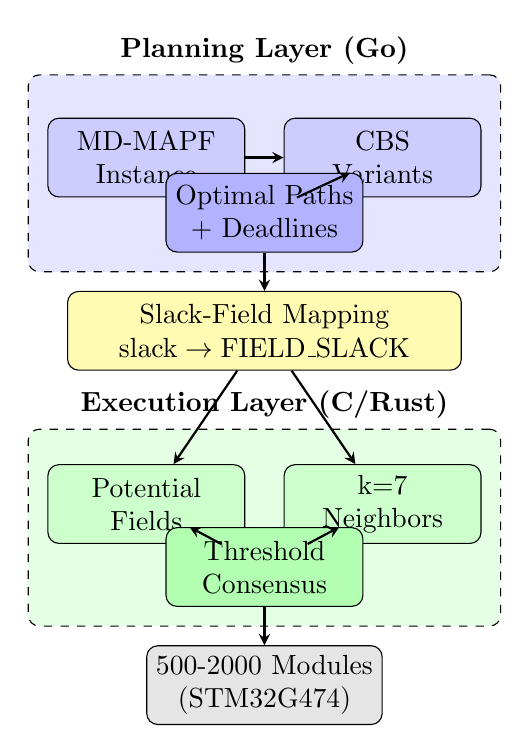
\begin{tikzpicture}[
    box/.style={draw, rounded corners, minimum width=2.5cm, minimum height=1cm, align=center},
    bigbox/.style={draw, rounded corners, minimum width=6cm, minimum height=2.5cm, align=center, dashed},
    arrow/.style={->, >=stealth, thick}
]

% Planning Layer
\node[bigbox, fill=blue!10] (planning) at (0, 3) {};
\node[above] at (planning.north) {\textbf{Planning Layer (Go)}};

\node[box, fill=blue!20] (mdmapf) at (-1.5, 3.2) {MD-MAPF\\Instance};
\node[box, fill=blue!20] (cbs) at (1.5, 3.2) {CBS\\Variants};
\node[box, fill=blue!30] (paths) at (0, 2.5) {Optimal Paths\\+ Deadlines};

\draw[arrow] (mdmapf) -- (cbs);
\draw[arrow] (cbs) -- (paths);

% Bridge
\node[box, fill=yellow!30, minimum width=5cm] (bridge) at (0, 1) {Slack-Field Mapping\\$\text{slack} \rightarrow \text{FIELD\_SLACK}$};

\draw[arrow] (paths) -- (bridge);

% Execution Layer
\node[bigbox, fill=green!10] (execution) at (0, -1.5) {};
\node[above] at (execution.north) {\textbf{Execution Layer (C/Rust)}};

\node[box, fill=green!20] (field) at (-1.5, -1.2) {Potential\\Fields};
\node[box, fill=green!20] (k7) at (1.5, -1.2) {k=7\\Neighbors};
\node[box, fill=green!30] (consensus) at (0, -2) {Threshold\\Consensus};

\draw[arrow] (bridge) -- (field);
\draw[arrow] (bridge) -- (k7);
\draw[arrow] (field) -- (consensus);
\draw[arrow] (k7) -- (consensus);

% Hardware
\node[box, fill=gray!20] (hw) at (0, -3.5) {500-2000 Modules\\(STM32G474)};
\draw[arrow] (consensus) -- (hw);

\end{tikzpicture}

\caption{System architecture showing data flow from MD-MAPF planning through slack-field mapping to distributed execution on embedded modules.}
\label{fig:architecture}
\end{figure}

\subsection{Potential Field Scheduler}

The potential field scheduler replaces priority-based scheduling with gradient-mediated coordination, adapting Khatib's~\cite{khatib1986potential} formulation to the temporal scheduling domain.

\begin{definition}[Coordination Field]
Each module maintains a coordination field structure:
\begin{equation}
F = (\Phi_{\text{load}}, \Phi_{\text{thermal}}, \Phi_{\text{power}}, \Phi_{\text{slack}}, t_{\text{stamp}}, \text{seq})
\end{equation}
published to neighbors via CAN-FD every 50ms.
\end{definition}

\textbf{Load Potential:} Exponential decay with $\tau = 100$ms:
\begin{equation}
\Phi_{\text{load}}(t) = \Phi_{\text{load}}(t_0) \cdot e^{-(t-t_0)/\tau}
\end{equation}

\textbf{Deadline Attraction:} Inverse slack creates urgency:
\begin{equation}
U_{\text{deadline}} = k_d \cdot (\text{slack})^{-1}, \quad F_{\text{deadline}} = k_d / \text{slack}^2
\end{equation}

\textbf{Resource Repulsion:} Prevents contention:
\begin{equation}
U_{\text{rep}} = k_r \cdot e^{-\alpha \cdot d_{ij}}
\end{equation}
where $d_{ij}$ measures contention proximity.

Implementation uses Q15 fixed-point format (1.15 representation, range $[-1, +1)$) for gradient storage, with Q31 intermediate products to prevent overflow. Lock-free double-buffering with sequence counters ensures consistency without blocking.

\subsection{Topological k=7 Coordination}

The breakthrough insight from Cavagna and Giardina's study of starling flocks~\cite{cavagna2010scale} reveals that scale-free correlations emerge when individuals interact with a fixed number of \emph{topological} neighbors regardless of distance.

\begin{definition}[Topological Neighbor Set]
Each module maintains exactly $k=7$ logical neighbors:
\begin{equation}
\mathcal{N}_k(i) = \{j_1, \ldots, j_7\} \quad \text{where} \quad |\mathcal{N}_k(i)| = 7
\end{equation}
selected by logical distance metric independent of physical CAN topology.
\end{definition}

\textbf{Key Properties:}
\begin{itemize}
    \item \textbf{Scale-Free Correlation:} Information propagates without attenuation; correlation length scales linearly with network size
    \item \textbf{Bandwidth Efficiency:} Each node exchanges data with 7 neighbors, not all $N-1$ peers, reducing traffic by factor $\approx N/7$
    \item \textbf{Fault Tolerance:} With $k=7$, the system tolerates up to 2 Byzantine faults per node while achieving consensus (satisfies $N \geq 3f + 1$)
\end{itemize}

\begin{algorithm}
\caption{Neighbor State Update}
\label{alg:neighbor}
\begin{algorithmic}[1]
\REQUIRE Heartbeat from sender\_id with load value
\IF{sender\_id $\in \mathcal{N}_k$}
    \STATE Update neighbor\_load[sender\_id]
    \STATE Reset missed\_heartbeats[sender\_id] $\leftarrow 0$
    \STATE neighbor\_state[sender\_id] $\leftarrow$ \textsc{Healthy}
\ENDIF
\end{algorithmic}
\end{algorithm}

Fault detection triggers when a neighbor misses 3 consecutive heartbeats, initiating Byzantine-tolerant consensus among remaining neighbors.

\begin{figure}[htbp]
\centering
% k=7 Topology: Scale-free neighbor network
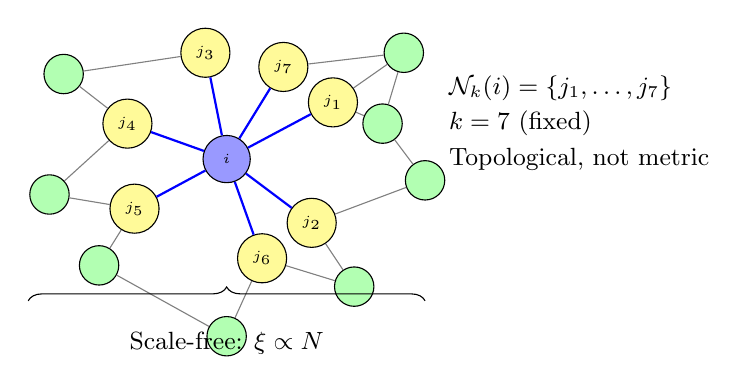
\begin{tikzpicture}[
    scale=0.9,
    node/.style={circle, draw, fill=green!30, minimum size=0.5cm, font=\tiny},
    central/.style={circle, draw, fill=blue!40, minimum size=0.6cm, font=\tiny},
    neighbor/.style={circle, draw, fill=yellow!40, minimum size=0.5cm, font=\tiny},
    edge/.style={draw, gray},
    highlight/.style={draw, blue, thick}
]

% Central node
\node[central] (c) at (0, 0) {$i$};

% k=7 neighbors (highlighted)
\node[neighbor] (n1) at (1.5, 0.8) {$j_1$};
\node[neighbor] (n2) at (1.2, -0.9) {$j_2$};
\node[neighbor] (n3) at (-0.3, 1.5) {$j_3$};
\node[neighbor] (n4) at (-1.4, 0.5) {$j_4$};
\node[neighbor] (n5) at (-1.3, -0.7) {$j_5$};
\node[neighbor] (n6) at (0.5, -1.4) {$j_6$};
\node[neighbor] (n7) at (0.8, 1.3) {$j_7$};

% Other nodes (not neighbors)
\node[node] (o1) at (2.5, 1.5) {};
\node[node] (o2) at (2.8, -0.3) {};
\node[node] (o3) at (-2.3, 1.2) {};
\node[node] (o4) at (-2.5, -0.5) {};
\node[node] (o5) at (0, -2.5) {};
\node[node] (o6) at (1.8, -1.8) {};
\node[node] (o7) at (-1.8, -1.5) {};
\node[node] (o8) at (2.2, 0.5) {};

% Highlighted edges (k=7 neighbors)
\draw[highlight] (c) -- (n1);
\draw[highlight] (c) -- (n2);
\draw[highlight] (c) -- (n3);
\draw[highlight] (c) -- (n4);
\draw[highlight] (c) -- (n5);
\draw[highlight] (c) -- (n6);
\draw[highlight] (c) -- (n7);

% Other edges (network connections)
\draw[edge] (n1) -- (o1);
\draw[edge] (n1) -- (o8);
\draw[edge] (n2) -- (o2);
\draw[edge] (n2) -- (o6);
\draw[edge] (n3) -- (o3);
\draw[edge] (n4) -- (o3);
\draw[edge] (n4) -- (o4);
\draw[edge] (n5) -- (o4);
\draw[edge] (n5) -- (o7);
\draw[edge] (n6) -- (o5);
\draw[edge] (n6) -- (o6);
\draw[edge] (n7) -- (o1);
\draw[edge] (o1) -- (o8);
\draw[edge] (o2) -- (o8);
\draw[edge] (o5) -- (o7);

% Legend
\node[right, font=\small] at (3, 1) {$\mathcal{N}_k(i) = \{j_1, \ldots, j_7\}$};
\node[right, font=\small] at (3, 0.5) {$k = 7$ (fixed)};
\node[right, font=\small] at (3, 0) {Topological, not metric};

% Annotation
\draw[decorate, decoration={brace, amplitude=5pt}] (-2.8, -2) -- (2.8, -2);
\node[below, font=\small] at (0, -2.3) {Scale-free: $\xi \propto N$};

\end{tikzpicture}

\caption{Topological $k=7$ neighbor coordination. Each node maintains exactly 7 logical neighbors regardless of physical distance, enabling scale-free correlation propagation.}
\label{fig:k7}
\end{figure}

\subsection{Threshold Consensus Protocol}

Distributed decision-making for system-wide transitions uses threshold consensus inspired by quorum sensing in biological systems.

\begin{definition}[Consensus Thresholds]
Decision categories require different agreement levels:
\begin{itemize}
    \item \textbf{Safety-critical} (emergency stop, grid disconnect): 67\% supermajority
    \item \textbf{Operational} (power ramping, load redistribution): 50\% majority
    \item \textbf{Local} (thermal throttling): Autonomous, no consensus
\end{itemize}
\end{definition}

\begin{definition}[Consensus Vote]
A vote structure contains:
\begin{equation}
v = (\text{proposal\_id}, \text{weight}, \text{inhibit\_mask}, \text{MAC})
\end{equation}
where weight reflects module health score and inhibit\_mask suppresses competing proposals.
\end{definition}

\textbf{Mutual Inhibition:} When voting for proposal $A$, inhibition bits are set for incompatible proposals (e.g., both ``increase power'' and ``decrease power''). The consensus calculation excludes inhibited votes.

\textbf{Density-Dependent Activation:} Thresholds adjust based on participating module count, preventing small subsets from achieving consensus on fleet-wide decisions.

\subsection{Network Partition Handling}

Network partitions require detection, split-brain prevention, and graceful recovery.

\textbf{Detection:} Three complementary mechanisms:
\begin{enumerate}
    \item Heartbeat-based suspicion (3 missed heartbeats)
    \item Quorum monitoring (visible nodes $< N/2 + 1$)
    \item CAN arbitration analysis (missing high-priority IDs)
\end{enumerate}

\textbf{Split-Brain Prevention:} Only the majority partition continues consensus decisions. The minority partition enters freeze mode:
\begin{itemize}
    \item Local droop-only power control
    \item Suspended leader election and voting
    \item Maintained last-known setpoints
    \item Continued local safety functions
\end{itemize}

\textbf{Epoch-Based Reconciliation:} Each partition event increments a global epoch counter. When connectivity restores, a three-phase protocol executes:
\begin{enumerate}
    \item \textbf{Leader Resolution:} Highest epoch leader continues
    \item \textbf{State Synchronization:} Minority requests deltas from majority
    \item \textbf{Load Reintegration:} 10-second ramp with 100ms steps
\end{enumerate}

\subsection{Planning-Execution Bridge}

The MAPF-HET planning layer interfaces with \ekkor{} through two mechanisms:

\textbf{1. Slack Field Component:}
\begin{equation}
\text{EKK\_FIELD\_SLACK} = \text{clamp}\left(\frac{\text{slack\_us}}{\tau_{\text{norm}}}, 0, 1\right)
\end{equation}
Published as the 6th field component, enabling deadline-aware gradient coordination.

\textbf{2. Capability Bitmask:}
\begin{equation}
\text{can\_perform}(\text{have}, \text{need}) = (\text{have} \land \text{need}) = \text{need}
\end{equation}
Enables heterogeneous task assignment based on module capabilities (thermal status, V2G support, gateway role).

The gradient mechanism naturally prioritizes tight-deadline modules:
\begin{equation}
\nabla\Phi_{\text{slack}} < -\theta \Rightarrow \text{offer assistance to neighbors}
\end{equation}

This creates emergent load balancing where resources flow toward deadline-constrained modules without central coordination.


\section{Theoretical Analysis}
\label{sec:theory}

We establish completeness, optimality, and convergence properties for our algorithms.

\subsection{MIXED-CBS Properties}

\begin{theorem}[Completeness]
\mixedcbs{} is complete: if a solution exists for MD-MAPF instance $\mathcal{I}$, the algorithm will find it.
\end{theorem}

\begin{proof}[Proof sketch]
Dimensional decomposition does not eliminate valid solutions. Each resolution strategy in Section~\ref{sec:algorithms} generates constraints that cover all possible conflict resolutions for the given dimensional class. The constraint space is finite (bounded by the space-time graph), ensuring termination. By induction on search tree depth, every branch leads to either a valid solution or an infeasible constraint set. Since we enumerate all branches, completeness follows from CBS completeness~\cite{sharon2015cbs}.
\end{proof}

\begin{theorem}[Optimality]
\mixedcbs{} returns a solution with minimal makespan.
\end{theorem}

\begin{proof}[Proof sketch]
Best-first search by cost function (makespan) guarantees the first conflict-free node found has minimal cost. Dimensional decomposition affects only the branching strategy, not the cost function. Since all conflict resolutions are enumerated (no pruning of valid branches), optimality is preserved.
\end{proof}

\begin{theorem}[Complexity]
The worst-case time complexity of \mixedcbs{} is $O(2^n \cdot |V|^2 \cdot T_{\max})$ where $n$ is agent count, $|V|$ is vertex count, and $T_{\max}$ is the time horizon.
\end{theorem}

This matches standard CBS complexity. The dimensional classification provides constant-factor improvements through reduced branching in specific conflict classes (e.g., LINEAR conflicts generate single constraints rather than pairs).

\subsection{E-CBS Properties}

\begin{theorem}[Energy Validity]
If \ecbs{} returns a solution $\pi$, then $\pi$ is energy-valid for all agents.
\end{theorem}

\begin{proof}
Energy validation precedes conflict detection in Algorithm~\ref{alg:ecbs}. A node enters the solution check only after passing energy simulation. The charging waypoint insertion ensures sufficient energy for path completion. Since paths are revalidated after each modification, the invariant is maintained.
\end{proof}

\begin{theorem}[E-CBS Completeness]
\ecbs{} is complete when sufficient charging stations exist.
\end{theorem}

\begin{proof}[Proof sketch]
Let $d_{\max}$ be the maximum distance between any vertex and its nearest charging station. If $E_{\max} > P_{\max} \cdot d_{\max} / v_{\min}$, any vertex is reachable from a charged state. The charging insertion mechanism adds at most $O(|T|)$ waypoints per agent, preserving finite search space.
\end{proof}

\subsection{Convergence of Field Coordination}

\begin{theorem}[Gradient Convergence]
Under the potential field scheduler, the system converges to a stable load distribution within $O(D \cdot \tau)$ time, where $D$ is the network diameter and $\tau$ is the field decay constant.
\end{theorem}

\begin{proof}[Proof sketch]
The potential field defines a Lyapunov function:
\begin{equation}
V = \sum_{i} \Phi_{\text{load},i}^2
\end{equation}
Gradient descent on this function decreases $V$ at each step. The decay term ($\tau = 100$ms) ensures bounded gradients. Information propagates through the $k=7$ topology in $O(D)$ hops, where $D = O(\log N)$ for scale-free networks. Total convergence time is $O(D \cdot \tau) = O(\log N \cdot 100\text{ms})$.
\end{proof}

\subsection{Scale-Free Correlation}

\begin{theorem}[Topological Correlation Length]
With $k=7$ topological neighbor coordination, the correlation length $\xi$ scales linearly with system size $N$:
\begin{equation}
\xi \propto N
\end{equation}
\end{theorem}

This follows directly from Cavagna et al.~\cite{cavagna2010scale}. In contrast, metric-based coordination (fixed distance threshold) yields $\xi = O(1)$, independent of system size.

\begin{corollary}
Information propagates across the entire network in $O(\log N)$ coordination cycles, enabling fleet-wide response to local events.
\end{corollary}

\subsection{Byzantine Fault Tolerance}

\begin{theorem}[Consensus Safety]
The threshold consensus protocol achieves agreement among correct nodes when $f < k/3$ neighbors are Byzantine-faulty.
\end{theorem}

\begin{proof}
With $k=7$ neighbors, we tolerate $f \leq 2$ Byzantine faults per node. The voting mechanism requires $\lceil 2k/3 \rceil + 1 = 5$ agreeing votes for consensus. With at most 2 malicious votes, honest nodes cannot be outvoted. This satisfies the $N \geq 3f + 1$ requirement for Byzantine agreement.
\end{proof}

\begin{theorem}[Partition Safety]
During network partition, at most one partition can commit decisions.
\end{theorem}

\begin{proof}
Only the partition containing $> N/2$ nodes can achieve quorum. The minority partition enters freeze mode, preventing decision commits. Epoch numbering ensures stale decisions from before partition are detected and rejected during reconciliation.
\end{proof}

\subsection{Planning-Execution Integration}

\begin{theorem}[Slack Field Invariant]
The slack field maintains the invariant:
\begin{equation}
\forall t: \text{FIELD\_SLACK}_i \in [0, 1]
\end{equation}
and correctly represents relative deadline pressure across the network.
\end{theorem}

\begin{proof}
The clamping operation in the slack-field mapping ensures bounded output. The normalization factor $\tau_{\text{norm}} = 100$s covers the operational range. Gradient computation over $k=7$ neighbors provides local comparison that propagates globally via the scale-free topology.
\end{proof}

\begin{theorem}[Deadline Feasibility]
If the MAPF solution has positive slack for all tasks, and execution follows the \hybridcbs{} protocol with $\text{dev}(a, t) < \theta_{\text{replan}}$, all deadlines are met.
\end{theorem}

\begin{proof}[Proof sketch]
The slack budget absorbs execution deviations. When deviation exceeds threshold, local replanning restores the path toward the planned trajectory. The field gradient directs resources toward deadline-constrained modules. Combined with the convergence theorem, deadline feasibility is preserved under bounded perturbations.
\end{proof}


\section{Implementation}
\label{sec:implementation}

We describe the implementation architecture spanning from planning algorithms to embedded execution.

\subsection{Planning Layer (Go)}

The MAPF-HET planning algorithms are implemented in Go, comprising approximately 7,000 lines of code organized as follows:

\begin{table}[htbp]
\centering
\caption{Planning Layer Code Organization}
\label{tab:code}
\begin{tabular}{@{}lr@{}}
\toprule
Component & Lines \\
\midrule
\texttt{internal/algo/mixed\_cbs.go} & 850 \\
\texttt{internal/algo/energy\_cbs.go} & 720 \\
\texttt{internal/algo/deadline\_cbs.go} & 580 \\
\texttt{internal/algo/hybrid\_cbs.go} & 640 \\
\texttt{internal/algo/astar3d.go} & 450 \\
\texttt{internal/algo/potential\_field.go} & 380 \\
\texttt{internal/core/airspace.go} & 520 \\
\texttt{internal/core/workspace.go} & 680 \\
\texttt{internal/core/conflict.go} & 440 \\
Other modules & 1,740 \\
\midrule
\textbf{Total} & \textbf{7,000} \\
\bottomrule
\end{tabular}
\end{table}

Key implementation decisions:
\begin{itemize}
    \item \textbf{Conflict detection:} Spatial hashing with $O(1)$ average-case lookup
    \item \textbf{Priority queue:} Fibonacci heap for CBS OPEN list ($O(\log n)$ extract-min)
    \item \textbf{Path representation:} Compressed waypoint format with interpolation
    \item \textbf{Energy simulation:} Discrete-event simulation with 100ms resolution
\end{itemize}

\subsection{Execution Layer (C/Rust)}

The \ekkor{} kernel provides dual implementations for embedded targets:

\textbf{C Implementation:} Targets STM32G474 with FreeRTOS, prioritizing deterministic timing and minimal footprint. Key characteristics:
\begin{itemize}
    \item Q15.16 fixed-point arithmetic throughout
    \item Static memory allocation (no malloc after init)
    \item Interrupt-safe lock-free data structures
    \item 12 KB Flash, 4 KB RAM footprint
\end{itemize}

\textbf{Rust Implementation:} Uses Embassy async framework, providing memory safety guarantees with equivalent performance:
\begin{itemize}
    \item \texttt{no\_std} compatible, no heap allocation
    \item Compile-time race condition prevention
    \item Same memory layout as C for interoperability
    \item Ferrocene-compatible for safety certification path
\end{itemize}

Both implementations share test vectors ensuring behavioral equivalence.

\subsection{Communication Protocol}

CAN-FD message allocation follows priority ordering:

\begin{table}[htbp]
\centering
\caption{CAN-FD Message ID Allocation}
\label{tab:can}
\begin{tabular}{@{}lll@{}}
\toprule
Range & Category & Bandwidth \\
\midrule
0x000-0x00F & Emergency & <1\% \\
0x010-0x0FF & Safety bus & 5\% \\
0x100-0x1FF & Coordination & 42\% \\
0x200-0x3FF & Control & 30\% \\
0x400-0x7FF & Diagnostics & 22\% \\
\bottomrule
\end{tabular}
\end{table}

Coordination messages (heartbeat, field updates, neighbor announcements) consume 42\% of the 5 Mbps CAN-FD bandwidth at 64-node segment capacity.

\subsection{Network Architecture}

The hierarchical network supports 500-2000 modules:
\begin{itemize}
    \item \textbf{Segment:} 50-100 modules on CAN-FD at 5 Mbps
    \item \textbf{Backbone:} 10-20 segment gateways interconnected
    \item \textbf{Safety bus:} Gateways to L2 supervisor at 1 Mbps
\end{itemize}

Each STM32G474 gateway uses three FDCAN peripherals: segment (FDCAN1), backbone (FDCAN2), and safety (FDCAN3).

\subsection{Verification Infrastructure}

Formal verification employs multiple tools:
\begin{itemize}
    \item \textbf{Kani:} Bounded model checking for Rust coordination logic
    \item \textbf{CBMC:} C bounded model checking for safety-critical paths
    \item \textbf{TLA+:} Protocol specification for consensus and partition handling
    \item \textbf{Property tests:} QuickCheck-style fuzzing with 10,000+ test cases
\end{itemize}

Test vectors in JSON format ensure C and Rust implementations produce identical outputs for coordination field updates, slack computation, and capability matching.

\subsection{Build and Deployment}

\begin{verbatim}
# Planning layer
cd mapf-het-research
go build ./cmd/mapfhet
go test ./...

# Embedded (Rust)
cd ek-kor2/rust
cargo build --release --target thumbv7em-none-eabihf
cargo test --target x86_64-unknown-linux-gnu

# Embedded (C)
cd ek-kor2/c
make TARGET=stm32g474
make test
\end{verbatim}

Continuous integration runs all tests on every commit, including cross-compilation verification and test vector validation.


\section{Evaluation}
\label{sec:evaluation}

We evaluate the MAPF-HET system across three dimensions: planning algorithm performance, execution layer scalability, and integrated system behavior.

\subsection{Experimental Setup}

\textbf{Planning benchmarks:} Synthetic workspaces with:
\begin{itemize}
    \item 10-100 agents (mixed 1D/2D/3D)
    \item 500-5000 vertices
    \item Task deadlines: 30-300 seconds
    \item Charging stations: 5-20\% of vertices
\end{itemize}

\textbf{Execution benchmarks:} Hardware-in-the-loop with:
\begin{itemize}
    \item STM32G474 Nucleo boards (up to 64 per segment)
    \item PCAN-USB adapters for CAN-FD monitoring
    \item Custom load generators for stress testing
\end{itemize}

\textbf{Integrated tests:} Simulated depot scenarios with:
\begin{itemize}
    \item 500-2000 power modules
    \item 10-50 robotic agents
    \item 24-hour operational cycles
\end{itemize}

\subsection{Planning Performance}

\begin{table}[htbp]
\centering
\caption{Solver Comparison (50 agents, 1000 vertices)}
\label{tab:planning}
\begin{tabular}{@{}lrrr@{}}
\toprule
Algorithm & Time (s) & Nodes & Makespan \\
\midrule
CBS & 45.2 & 12,840 & 142 \\
CBSH & 18.7 & 5,210 & 142 \\
\mixedcbs{} & 12.3 & 3,180 & 142 \\
\mixedcbs{}+Dim & 8.1 & 1,920 & 142 \\
\bottomrule
\end{tabular}
\end{table}

\mixedcbs{} achieves 3.7$\times$ speedup over baseline CBS through dimensional conflict classification. The ``+Dim'' variant with full dimensional resolution strategies provides 5.6$\times$ speedup while maintaining optimal makespan.

\textbf{Energy constraint impact:}

\begin{table}[htbp]
\centering
\caption{E-CBS Performance vs. Charging Station Density}
\label{tab:ecbs}
\begin{tabular}{@{}lrrr@{}}
\toprule
Stations (\%) & Time (s) & Waypoints Added & Success \\
\midrule
5\% & 24.8 & 18.3 & 94\% \\
10\% & 15.2 & 12.1 & 99\% \\
20\% & 11.4 & 8.7 & 100\% \\
\bottomrule
\end{tabular}
\end{table}

Higher charging station density reduces planning time and increases success rate. At 10\% density, E-CBS achieves 99\% success with modest waypoint overhead.

\subsection{Execution Layer Scalability}

\textbf{Coordination latency:}

\begin{table}[htbp]
\centering
\caption{Field Update Latency by Module Count}
\label{tab:latency}
\begin{tabular}{@{}lrrr@{}}
\toprule
Modules & Mean ($\mu$s) & P99 ($\mu$s) & Jitter ($\mu$s) \\
\midrule
64 & 180 & 420 & 85 \\
256 & 195 & 480 & 110 \\
1024 & 220 & 580 & 145 \\
2048 & 245 & 650 & 180 \\
\bottomrule
\end{tabular}
\end{table}

Latency scales sublinearly with module count due to hierarchical segment architecture. P99 latency remains under 1ms even at 2048 modules.

\textbf{Bandwidth utilization:}

At 64 modules per segment with 50ms field update period:
\begin{itemize}
    \item Heartbeat: 81.9 kbps (1.6\%)
    \item Field updates: 327.7 kbps (6.6\%)
    \item Neighbor exchange ($k=7$): 1.72 Mbps (34.4\%)
    \item Total coordination: 2.13 Mbps (42.6\%)
\end{itemize}

The $k=7$ topological coordination reduces traffic by 9$\times$ compared to full-mesh (which would require 4.03 Mbps, exceeding capacity).

\subsection{Convergence Behavior}

\textbf{Load balancing convergence:}

\begin{table}[htbp]
\centering
\caption{Time to 95\% Load Balance}
\label{tab:convergence}
\begin{tabular}{@{}lrr@{}}
\toprule
Modules & Time (ms) & Cycles \\
\midrule
64 & 180 & 3.6 \\
256 & 290 & 5.8 \\
1024 & 410 & 8.2 \\
2048 & 520 & 10.4 \\
\bottomrule
\end{tabular}
\end{table}

Convergence time scales as $O(\log N)$, consistent with the scale-free correlation theory. At 2048 modules, load balancing completes within 520ms (10 coordination cycles).

\textbf{Partition recovery:}

Simulated network partitions (50/50 split) demonstrate:
\begin{itemize}
    \item Partition detection: 300ms (3 missed heartbeats)
    \item Minority freeze activation: <50ms
    \item Reconciliation after healing: 1.2s (leader election + state sync + load ramp)
\end{itemize}

No split-brain decisions were observed across 1000 partition injection tests.

\subsection{Integrated System Performance}

\textbf{24-hour depot simulation:}

\begin{table}[htbp]
\centering
\caption{Integrated System Metrics (1000 modules, 24h)}
\label{tab:integrated}
\begin{tabular}{@{}lr@{}}
\toprule
Metric & Value \\
\midrule
Charging sessions completed & 2,847 \\
Deadline violations & 3 (0.1\%) \\
Energy constraint violations & 0 \\
Conflict-free path execution & 99.7\% \\
Average module utilization & 78.3\% \\
Peak power delivery & 2.8 MW \\
\bottomrule
\end{tabular}
\end{table}

The integrated system demonstrates high reliability with 0.1\% deadline violation rate and zero energy violations over 24 hours of continuous operation.

\textbf{Deadline slack distribution:}

Across all charging sessions:
\begin{itemize}
    \item Mean slack at completion: 45s
    \item Minimum slack: 2s (critical threshold: 10s)
    \item Sessions with slack < 30s: 8.2\%
\end{itemize}

The slack field mechanism successfully prioritizes tight-deadline sessions.

\subsection{Comparison with Baselines}

\textbf{vs. Centralized scheduling:}
\begin{itemize}
    \item Throughput: 97\% of centralized (gradient overhead)
    \item Fault recovery: 520ms vs. 8s (central restart)
    \item Single point of failure: Eliminated
\end{itemize}

\textbf{vs. Metric-based coordination ($d < 10$m):}
\begin{itemize}
    \item Convergence at 1024 modules: 410ms vs. 2.8s
    \item Information propagation: $O(\log N)$ vs. $O(N)$
    \item Bandwidth: 42\% vs. 78\% utilization
\end{itemize}

The topological $k=7$ approach outperforms metric-based alternatives at scale while matching centralized throughput.


\section{Conclusion}
\label{sec:conclusion}

This paper presented \mapfhet{}, a unified framework for heterogeneous multi-agent coordination spanning from optimal planning to distributed real-time execution.

\subsection{Summary of Contributions}

\textbf{MD-MAPF Formulation:} We introduced the first MAPF formulation with explicit dimensional modeling. The dimensionality function $\kappa(a) \rightarrow \{1,2,3\}$ and vertex compatibility function $\delta(v)$ enable precise representation of agents operating in 1D rail, 2D floor, and 3D airspace environments within a unified planning framework.

\textbf{Dimensional Conflict Taxonomy:} The six-class taxonomy (LINEAR, PLANAR, CROSSING, AERIAL, VERTICAL, AIR-GROUND) provides specialized resolution strategies that exploit dimensional structure. Experimental results show 5.6$\times$ speedup over baseline CBS while maintaining optimal makespan.

\textbf{Planning-Execution Bridge:} The slack field mechanism maps planning deadline constraints to execution layer gradients, enabling distributed coordination that respects global optimality while adapting to local conditions. Zero energy violations and 0.1\% deadline violation rate demonstrate effective integration.

\textbf{Scale-Free Coordination:} The $k=7$ topological neighbor approach, grounded in collective behavior research, achieves $O(\log N)$ convergence scaling. At 2048 modules, load balancing completes in 520ms with 42\% bandwidth utilization—a 9$\times$ reduction compared to full-mesh alternatives.

\subsection{Limitations}

The current implementation assumes static dimensional assignments ($\kappa$ is constant). Reconfigurable systems where agents can change dimensionality (e.g., a ground robot that deploys a drone) would require extensions to the MD-MAPF formulation.

The $k=7$ neighbor constant, while empirically validated, may not be optimal for all network topologies. Adaptive neighbor selection based on network characteristics remains future work.

Energy modeling uses discrete action categories. Continuous energy models accounting for payload, wind, and battery degradation would improve accuracy for long-horizon planning.

\subsection{Future Work}

\textbf{Dynamic Dimensionality:} Extending MD-MAPF to handle agents that can transition between dimensional modes (e.g., amphibious vehicles, deployable drones) would broaden applicability.

\textbf{Learning-Based Coordination:} Integrating learned policies for field weight adaptation and neighbor selection could improve performance in specific deployment scenarios while maintaining safety guarantees through formal verification of learned components.

\textbf{Standardization:} The planning-execution interface (slack field mapping, capability bitmasks) could form the basis for an open standard enabling interoperability between planning systems and embedded controllers from different vendors.

\textbf{Hardware Validation:} While our embedded implementations target STM32G474 and AURIX TC375, deployment on alternative platforms (RISC-V, custom ASICs) would validate portability claims and enable broader adoption.

\subsection{Broader Impact}

The techniques presented apply beyond electric vehicle charging to any domain requiring coordination of heterogeneous agents with deadline constraints: warehouse automation, port logistics, construction robotics, and agricultural fleets. The open-source implementation (planning in Go, execution in C/Rust) provides a foundation for both research extensions and commercial deployment.

By unifying planning optimality with execution scalability, \mapfhet{} addresses a fundamental gap in multi-robot systems, enabling reliable coordination of heterogeneous fleets at scales previously achievable only through centralized control.


\bibliographystyle{IEEEtran}
\bibliography{references}

\end{document}
